\documentclass[11pt, a4paper]{article}

% Fonts and Encoding
\usepackage[utf8]{inputenc}
\usepackage[T1]{fontenc}

% Math and Symbols
\usepackage{amsmath, amssymb, amsthm, amsfonts, mathrsfs, mathtools}

% Layout and Geometry
\usepackage{geometry}
\geometry{a4paper, margin=1in}

% Formatting and Graphics
\usepackage{graphicx, xcolor, enumitem, booktabs, array, tabularx}

% TikZ for Illustrations
\usepackage{tikz}
\usetikzlibrary{arrows.meta, positioning, shapes.geometric, calc, backgrounds, matrix}

% Clickable Links and TOC
\usepackage{hyperref}
\hypersetup{
    colorlinks=true,
    linkcolor=blue,
    filecolor=magenta,      
    urlcolor=cyan,
    pdftitle={Advanced Mathematics: Moment-Generating Functions and Tail Bounds},
}

% Theorem Environments
\newtheorem{theorem}{Theorem}[section]
\newtheorem{lemma}[theorem]{Lemma}
\newtheorem{proposition}[theorem]{Proposition}
\newtheorem{corollary}[theorem]{Corollary}
\theoremstyle{definition}
\newtheorem{definition}{Definition}[section]
\newtheorem{axiom}{Axiom}[section]
\newtheorem{example}{Example}[section]
\theoremstyle{remark}
\newtheorem{remark}{Remark}[section]

% Custom Commands (Enforced standard notation)
\newcommand{\R}{\mathbb{R}}
\newcommand{\N}{\mathbb{N}}
\newcommand{\Z}{\mathbb{Z}}
\newcommand{\Q}{\mathbb{Q}}
\newcommand{\E}{\mathbb{E}}
\newcommand{\Prob}{\mathbb{P}}
\newcommand{\F}{\mathcal{F}}

\begin{document}

\title{\textbf{Advanced Mathematics: Moment-Generating Functions, Tail Bounds, and Theoretical Probability}}
\author{Tashfeen Omran}
\date{October 29, 2026}
\maketitle

\tableofcontents
\newpage

\section{Concept Checklist \& Question Mapping}

The following table maps the theoretical concepts, logical structures, and proof techniques extracted from the source text to the corresponding problems in this document.

\renewcommand{\arraystretch}{1.5}
\begin{table}[h!]
\centering
\begin{tabularx}{\textwidth}{>{\raggedright\arraybackslash}p{0.7\textwidth} >{\centering\arraybackslash}X}
\toprule
\textbf{Theoretical Concept / Proof Technique} & \textbf{Problem(s)} \\
\midrule
C1: MGF Derivation \& Convergence Constraints (Improper Integrals) & 1, 2, 4 \\
C2: Moment Extraction via Differentiation ($k$-th derivative) & 5, 30 \\
C3: Linear Transformations of MGFs & 6, 7 \\
C4: Distribution Identification via Isomorphism (Uniqueness Theorem) & 9, 10 \\
C5: Tchebysheff's Theorem for Interval Estimation & 13 \\
C6: Tchebysheff's Theorem for Variance Constraints & 14 \\
C7: Tchebysheff vs. Exact Probability (Uniform, Normal, Exponential) & 15, 30 \\
C8: Chernoff Bounds (Exponential tail bounds, Markov's Inequality) & 16, 17, 19 \\
C9: Abstract Real-World Modeling (PAC Learning, VaR, Quant Finance) & 21, 22, 23 \\
C10: Diagnostic Testing (Existence, Exactness, Independence, LOTUS) & 3, 8, 24, 25, 26, 27 \\
C11: Set-Theoretic \& Measure-Theoretic Foundations & 11, 12, 18, 20, 28, 29 \\
\bottomrule
\end{tabularx}
\end{table}

\newpage

\section{Problem Set: Theoretical Probability and Proofs}

\subsection{MGF Derivations, Convergence, and Moments}
\begin{enumerate}[label=\textbf{\arabic*.}]
    \item \textbf{Prove that} the Moment-Generating Function (MGF) of an Exponential random variable $Y \sim \text{Exp}(\lambda)$ is $m_Y(t) = \frac{\lambda}{\lambda - t}$, and explicitly state the convergence constraint on $t$.
    \item \textbf{Derive the probability measure} (MGF) for a Standard Normal random variable $Z \sim \mathcal{N}(0,1)$. 
    \item \textbf{Find a counterexample to} the Existence Fallacy: Prove rigorously that the standard Cauchy distribution, $f(y) = \frac{1}{\pi(1+y^2)}$, does not possess a valid MGF for any $t \neq 0$.
    \item \textbf{Derive} the MGF of the Laplace distribution with density $f(y) = \frac{\lambda}{2} e^{-\lambda|y|}$ for $y \in \R$.
    \item \textbf{Prove that} if the MGF $m_Y(t)$ exists for $|t| < b$, the $k$-th moment of $Y$ is given by $\E[Y^k] = \left. \frac{d^k}{dt^k} m_Y(t) \right|_{t=0}$.
\end{enumerate}

\subsection{Linear Transformations and the Uniqueness Theorem}
\begin{enumerate}[label=\textbf{\arabic*.}, resume]
    \item \textbf{Establish the logical equivalence} of linear transformations in the frequency domain: Prove that if $U = aY + b$, then $m_U(t) = e^{bt} m_Y(at)$.
    \item \textbf{Prove that} the sum of two independent normal random variables $X \sim \mathcal{N}(\mu_1, \sigma_1^2)$ and $Y \sim \mathcal{N}(\mu_2, \sigma_2^2)$ is also normally distributed, using the Uniqueness Theorem.
    \item \textbf{Find a counterexample to} the Independence Assumption Fallacy: Show that $m_{X+Y}(t) = m_X(t)m_Y(t)$ fails if $X$ and $Y$ are perfectly correlated (e.g., $Y = X$).
    \item \textbf{Identify the distribution} of a random variable $X$ whose MGF is $m_X(t) = \left(\frac{1}{3} + \frac{2}{3}e^t\right)^5$.
    \item \textbf{Prove that} the sum of $n$ independent Poisson random variables with parameters $\lambda_1, \dots, \lambda_n$ is a Poisson random variable with parameter $\sum_{i=1}^n \lambda_i$.
\end{enumerate}

\subsection{Measure-Theoretic Bounds: Markov and Tchebysheff}
\begin{enumerate}[label=\textbf{\arabic*.}, resume]
    \item \textbf{Prove} Markov's Inequality: For any non-negative continuous random variable $X$ and $a > 0$, $\Prob(X \ge a) \le \frac{\E[X]}{a}$.
    \item \textbf{Prove} Tchebysheff's Theorem using Markov's Inequality.
    \item \textbf{Interval Estimation:} A machine produces components with a mean lifespan of $\mu = 10,000$ hours and a standard deviation of $\sigma = 500$ hours. Using Tchebysheff's Theorem, find a symmetric interval around the mean that guarantees at least $84\%$ of the components fall within it.
    \item \textbf{Variance Constraints:} A chemical process yields a mean output of $\mu = 50$ liters. The manufacturer requires the output to be within $2$ liters of $\mu$ at least $88.89\%$ of the time. What is the maximum allowable variance $\sigma^2$?
    \item \textbf{Compare} the exact probability $\Prob(|Y - \mu| \le 2\sigma)$ for an Exponential distribution $Y \sim \text{Exp}(\lambda)$ against the theoretical lower bound provided by Tchebysheff's Theorem.
\end{enumerate}

\subsection{Advanced Tail Bounds: Chernoff and Hoeffding}
\begin{enumerate}[label=\textbf{\arabic*.}, resume]
    \item \textbf{Derive} the Chernoff Bound for a Standard Normal random variable $Z \sim \mathcal{N}(0,1)$ for the tail event $\Prob(Z \ge a)$ where $a > 0$.
    \item \textbf{Derive} the Chernoff Bound for a Poisson random variable $Y \sim \text{Poi}(\lambda)$ for the event $\Prob(Y \ge a)$ where $a > \lambda$.
    \item \textbf{Establish the logical equivalence} of the events $\{Y \ge a\}$ and $\{e^{tY} \ge e^{ta}\}$ for any $t > 0$, and explain its measure-theoretic significance in deriving the Chernoff bound.
    \item \textbf{Prove} Hoeffding's Lemma for a Rademacher random variable (where $\Prob(X=1) = 0.5$ and $\Prob(X=-1) = 0.5$): Show that $\E[e^{tX}] \le e^{t^2/2}$.
    \item \textbf{Prove} the one-sided Tchebysheff Inequality (Cantelli's Inequality): $\Prob(Y - \mu \ge a) \le \frac{\sigma^2}{\sigma^2 + a^2}$ for $a > 0$.
\end{enumerate}

\subsection{Abstract Real-World Modeling (AI, ML, \& Quant Finance)}
\begin{enumerate}[label=\textbf{\arabic*.}, resume]
    \item \textbf{PAC Learning (AI):} Let $\hat{L}(h)$ be the empirical risk of a classifier over $n$ samples, and $L(h)$ be the true risk. Given Hoeffding's Inequality $\Prob(|\hat{L}(h) - L(h)| \ge \epsilon) \le 2\exp(-2n\epsilon^2)$, derive the minimum sample size $n$ required to guarantee that the empirical risk is within $\epsilon = 0.05$ of the true risk with a probability of at least $1 - \delta$, where $\delta = 0.01$.
    \item \textbf{Algorithmic Trading (VaR):} A hedge fund's daily return $R$ has an unknown distribution with mean $\mu = 0.001$ and standard deviation $\sigma = 0.02$. Using Tchebysheff's Theorem, find the worst-case Value at Risk (VaR) threshold $V$ such that the probability of a loss greater than $V$ is at most $5\%$.
    \item \textbf{Quantitative Finance:} In a simplified jump-diffusion model, an asset's log-return is $X = Z + \sum_{i=1}^N Y_i$, where $Z \sim \mathcal{N}(\mu, \sigma^2)$, $N \sim \text{Poi}(\lambda)$, and $Y_i \sim \mathcal{N}(0, \delta^2)$. Assuming all variables are independent, derive the MGF of $X$.
\end{enumerate}

\subsection{Diagnostic Testing: "Find the Flaw" and Set Theory}
\begin{enumerate}[label=\textbf{\arabic*.}, resume]
    \item \textbf{Find the Flaw (Vacuous Bounds):} A student uses Tchebysheff's Theorem to bound the probability that a random variable deviates from its mean by $0.5\sigma$, concluding $\Prob(|Y - \mu| \ge 0.5\sigma) \le 4$. Explain the mathematical vacuousness of this result.
    \item \textbf{Find the Flaw (LOTUS Violation):} A researcher claims that since $m_X(t) = \E[e^{tX}]$, they can find $\E[1/X]$ by evaluating $m_X(-1) = \E[e^{-X}]$. Prove rigorously why this violates the Law of the Unconscious Statistician.
    \item \textbf{Find the Flaw (Uniqueness Conditions):} Two random variables $X$ and $Y$ have MGFs such that $m_X(1) = m_Y(1) = 5$. A student concludes $X$ and $Y$ have the same distribution. State the exact condition of the Uniqueness Theorem that is violated.
    \item \textbf{Find the Flaw (Convergence):} A student integrates $\int_0^\infty e^{ty} \frac{1}{y^2} dy$ and claims to have found an MGF. Identify the analytical error.
    \item \textbf{Measure Theory:} Prove the Continuity of Probability Measure from Below: If $A_1 \subseteq A_2 \subseteq \dots$ is an increasing sequence of events in a $\sigma$-algebra $\F$, then $\Prob(\bigcup_{i=1}^\infty A_i) = \lim_{n \to \infty} \Prob(A_n)$.
    \item \textbf{Measure Theory:} Prove the First Borel-Cantelli Lemma: If $\sum_{n=1}^\infty \Prob(A_n) < \infty$, then the probability that infinitely many $A_n$ occur is zero.
    \item \textbf{Conceptual Synthesis:} Let $Y$ follow a Laplace distribution with $\lambda = 1$. (a) Find the exact probability $\Prob(Y \ge 3)$. (b) Find the Tchebysheff bound for $\Prob(|Y| \ge 3)$. (c) Find the Chernoff bound for $\Prob(Y \ge 3)$. Compare the tightness of the bounds.
\end{enumerate}

\newpage

\section{Detailed Solutions}

\begin{proof}[\textbf{Solution to Problem 1}]
By definition, the MGF is $m_Y(t) = \E[e^{tY}]$. For $Y \sim \text{Exp}(\lambda)$, the PDF is $f(y) = \lambda e^{-\lambda y}$ for $y > 0$.
\begin{align*}
m_Y(t) &= \int_{0}^{\infty} e^{ty} \lambda e^{-\lambda y} \, dy \\
&= \lambda \int_{0}^{\infty} e^{-y(\lambda - t)} \, dy
\end{align*}
For this improper integral to converge, the exponent must be strictly negative, requiring $\lambda - t > 0 \implies t < \lambda$. Assuming this holds:
\begin{align*}
m_Y(t) &= \lambda \left[ \frac{e^{-y(\lambda - t)}}{-(\lambda - t)} \right]_{0}^{\infty} \\
&= \lambda \left( 0 - \frac{1}{-(\lambda - t)} \right) = \frac{\lambda}{\lambda - t}
\end{align*}
\end{proof}

\begin{proof}[\textbf{Solution to Problem 2}]
For $Z \sim \mathcal{N}(0,1)$, the PDF is $f(z) = \frac{1}{\sqrt{2\pi}} e^{-z^2/2}$.
\begin{align*}
m_Z(t) &= \int_{-\infty}^{\infty} e^{tz} \frac{1}{\sqrt{2\pi}} e^{-z^2/2} \, dz \\
&= \frac{1}{\sqrt{2\pi}} \int_{-\infty}^{\infty} \exp\left( -\frac{1}{2}(z^2 - 2tz) \right) \, dz
\end{align*}
Complete the square in the exponent: $z^2 - 2tz = (z - t)^2 - t^2$.
\begin{align*}
m_Z(t) &= \frac{1}{\sqrt{2\pi}} \int_{-\infty}^{\infty} \exp\left( -\frac{1}{2}((z - t)^2 - t^2) \right) \, dz \\
&= e^{t^2/2} \int_{-\infty}^{\infty} \frac{1}{\sqrt{2\pi}} \exp\left( -\frac{1}{2}(z - t)^2 \right) \, dz
\end{align*}
The integral represents the total probability mass of a $\mathcal{N}(t, 1)$ distribution, which equals $1$. Thus, $m_Z(t) = e^{t^2/2}$.
\end{proof}

\begin{proof}[\textbf{Solution to Problem 3}]
The MGF is defined as $\E[e^{tY}] = \int_{-\infty}^{\infty} e^{ty} \frac{1}{\pi(1+y^2)} \, dy$. 
Assume $t > 0$. As $y \to \infty$, the exponential term $e^{ty}$ grows infinitely faster than the polynomial term $1+y^2$. By L'H\^{o}pital's rule, $\lim_{y \to \infty} \frac{e^{ty}}{1+y^2} = \infty$. Therefore, the integrand does not approach zero, and the improper integral diverges to $\infty$. By symmetry, if $t < 0$, the integral diverges as $y \to -\infty$. Thus, the MGF only exists at $t=0$ (where it equals 1), meaning the Cauchy distribution has no valid MGF.
\end{proof}

\begin{proof}[\textbf{Solution to Problem 4}]
For the Laplace distribution, $f(y) = \frac{\lambda}{2} e^{-\lambda|y|}$.
\begin{align*}
m_Y(t) &= \int_{-\infty}^{\infty} e^{ty} \frac{\lambda}{2} e^{-\lambda|y|} \, dy \\
&= \frac{\lambda}{2} \int_{-\infty}^{0} e^{ty} e^{\lambda y} \, dy + \frac{\lambda}{2} \int_{0}^{\infty} e^{ty} e^{-\lambda y} \, dy \\
&= \frac{\lambda}{2} \int_{-\infty}^{0} e^{y(t+\lambda)} \, dy + \frac{\lambda}{2} \int_{0}^{\infty} e^{-y(\lambda-t)} \, dy
\end{align*}
For convergence, we require $t+\lambda > 0 \implies t > -\lambda$ and $\lambda-t > 0 \implies t < \lambda$. Thus, $|t| < \lambda$.
\begin{align*}
m_Y(t) &= \frac{\lambda}{2} \left[ \frac{1}{t+\lambda} \right] + \frac{\lambda}{2} \left[ \frac{1}{\lambda-t} \right] \\
&= \frac{\lambda}{2} \left( \frac{\lambda-t + t+\lambda}{\lambda^2 - t^2} \right) = \frac{\lambda^2}{\lambda^2 - t^2}
\end{align*}
\end{proof}

\begin{proof}[\textbf{Solution to Problem 5}]
By definition, $m_Y(t) = \E[e^{tY}]$. Using the Taylor series expansion of $e^{tY}$:
\[ e^{tY} = \sum_{k=0}^{\infty} \frac{(tY)^k}{k!} = 1 + tY + \frac{t^2Y^2}{2!} + \frac{t^3Y^3}{3!} + \dots \]
By the linearity of expectation (assuming conditions for interchanging expectation and summation hold):
\[ m_Y(t) = 1 + t\E[Y] + \frac{t^2}{2!}\E[Y^2] + \frac{t^3}{3!}\E[Y^3] + \dots \]
Taking the $k$-th derivative with respect to $t$:
\[ \frac{d^k}{dt^k} m_Y(t) = \E[Y^k] + t\E[Y^{k+1}] + \frac{t^2}{2!}\E[Y^{k+2}] + \dots \]
Evaluating at $t=0$, all terms containing $t$ vanish, leaving exactly $\E[Y^k]$.
\end{proof}

\begin{proof}[\textbf{Solution to Problem 6}]
Let $U = aY + b$. By the definition of the MGF and the linearity of expectation:
\begin{align*}
m_U(t) &= \E[e^{tU}] = \E[e^{t(aY+b)}] \\
&= \E[e^{atY} e^{bt}]
\end{align*}
Since $e^{bt}$ is a deterministic constant with respect to the random variable $Y$, it factors out:
\[ m_U(t) = e^{bt} \E[e^{(at)Y}] = e^{bt} m_Y(at) \]
\end{proof}

\begin{proof}[\textbf{Solution to Problem 7}]
Let $X \sim \mathcal{N}(\mu_1, \sigma_1^2)$ and $Y \sim \mathcal{N}(\mu_2, \sigma_2^2)$ be independent. Their MGFs are $m_X(t) = \exp(\mu_1 t + \frac{1}{2}\sigma_1^2 t^2)$ and $m_Y(t) = \exp(\mu_2 t + \frac{1}{2}\sigma_2^2 t^2)$.
Because $X$ and $Y$ are independent, the MGF of their sum is the product of their MGFs:
\begin{align*}
m_{X+Y}(t) &= m_X(t) m_Y(t) \\
&= \exp\left(\mu_1 t + \frac{1}{2}\sigma_1^2 t^2\right) \exp\left(\mu_2 t + \frac{1}{2}\sigma_2^2 t^2\right) \\
&= \exp\left( (\mu_1 + \mu_2)t + \frac{1}{2}(\sigma_1^2 + \sigma_2^2)t^2 \right)
\end{align*}
This matches the canonical MGF form of a Normal distribution with mean $\mu_1+\mu_2$ and variance $\sigma_1^2+\sigma_2^2$. By the Uniqueness Theorem, $X+Y \sim \mathcal{N}(\mu_1+\mu_2, \sigma_1^2+\sigma_2^2)$.
\end{proof}

\begin{proof}[\textbf{Solution to Problem 8}]
Let $X \sim \mathcal{N}(0,1)$. Suppose $Y = X$. Then $X$ and $Y$ are perfectly dependent.
The sum is $X+Y = 2X$. The true MGF of the sum is:
\[ m_{2X}(t) = \E[e^{t(2X)}] = m_X(2t) = \exp\left(\frac{(2t)^2}{2}\right) = \exp(2t^2) \]
However, if we falsely assume $m_{X+Y}(t) = m_X(t)m_Y(t)$, we get:
\[ m_X(t)m_X(t) = \exp(t^2/2) \exp(t^2/2) = \exp(t^2) \]
Since $\exp(2t^2) \neq \exp(t^2)$ for $t \neq 0$, the multiplicative property fails without independence.
\end{proof}

\begin{proof}[\textbf{Solution to Problem 9}]
The given MGF is $m_X(t) = \left(\frac{1}{3} + \frac{2}{3}e^t\right)^5$.
Recall the MGF of a Binomial distribution $Y \sim \text{Bin}(n, p)$ is $m_Y(t) = (1-p + pe^t)^n$.
By algebraic pattern matching, we identify $n = 5$, $p = 2/3$, and $1-p = 1/3$.
By the Uniqueness Theorem, $X$ must follow a Binomial distribution: $X \sim \text{Bin}(5, 2/3)$.
\end{proof}

\begin{proof}[\textbf{Solution to Problem 10}]
Let $X_i \sim \text{Poi}(\lambda_i)$ be independent. The MGF of a Poisson random variable is $m_{X_i}(t) = \exp(\lambda_i(e^t - 1))$.
Let $S = \sum_{i=1}^n X_i$. By independence:
\begin{align*}
m_S(t) &= \prod_{i=1}^n m_{X_i}(t) = \prod_{i=1}^n \exp(\lambda_i(e^t - 1)) \\
&= \exp\left( \sum_{i=1}^n \lambda_i(e^t - 1) \right) = \exp\left( (e^t - 1) \sum_{i=1}^n \lambda_i \right)
\end{align*}
This is the MGF of a Poisson distribution with parameter $\Lambda = \sum_{i=1}^n \lambda_i$. By the Uniqueness Theorem, $S \sim \text{Poi}(\sum \lambda_i)$.
\end{proof}

\begin{proof}[\textbf{Solution to Problem 11}]
Let $X$ be a continuous non-negative random variable with PDF $f(x)$. By definition:
\[ \E[X] = \int_{0}^{\infty} x f(x) \, dx \]
Split the integral at $a > 0$:
\[ \E[X] = \int_{0}^{a} x f(x) \, dx + \int_{a}^{\infty} x f(x) \, dx \]
Since $X \ge 0$, the first integral is non-negative. Thus:
\[ \E[X] \ge \int_{a}^{\infty} x f(x) \, dx \]
In the region of integration $[a, \infty)$, $x \ge a$. Therefore:
\[ \E[X] \ge \int_{a}^{\infty} a f(x) \, dx = a \int_{a}^{\infty} f(x) \, dx = a \Prob(X \ge a) \]
Dividing by $a$ yields $\Prob(X \ge a) \le \frac{\E[X]}{a}$.
\end{proof}

\begin{proof}[\textbf{Solution to Problem 12}]
We wish to bound $\Prob(|Y - \mu| \ge k\sigma)$.
Notice that the event $\{|Y - \mu| \ge k\sigma\}$ is logically and set-theoretically identical to the event $\{(Y - \mu)^2 \ge k^2\sigma^2\}$.
Let $X = (Y - \mu)^2$. Since $X$ is strictly non-negative, we can apply Markov's Inequality with $a = k^2\sigma^2$:
\[ \Prob(X \ge a) \le \frac{\E[X]}{a} \]
Substitute $X$ and $a$:
\[ \Prob((Y - \mu)^2 \ge k^2\sigma^2) \le \frac{\E[(Y - \mu)^2]}{k^2\sigma^2} \]
By definition, $\E[(Y - \mu)^2] = \sigma^2$. Thus:
\[ \Prob(|Y - \mu| \ge k\sigma) \le \frac{\sigma^2}{k^2\sigma^2} = \frac{1}{k^2} \]
\end{proof}

\begin{proof}[\textbf{Solution to Problem 13}]
We require an interval $[\mu - k\sigma, \mu + k\sigma]$ that contains at least $84\%$ of the probability mass. This means the probability of falling outside the interval is at most $16\%$.
\[ \Prob(|Y - \mu| \ge k\sigma) \le 0.16 \]
By Tchebysheff's Theorem, $\Prob(|Y - \mu| \ge k\sigma) \le \frac{1}{k^2}$. We set the bound:
\[ \frac{1}{k^2} = 0.16 \implies k^2 = \frac{1}{0.16} = 6.25 \implies k = 2.5 \]
The interval is $\mu \pm 2.5\sigma = 10000 \pm 2.5(500) = 10000 \pm 1250$.
The interval is $[8750, 11250]$ hours.
\end{proof}

\begin{proof}[\textbf{Solution to Problem 14}]
We require $\Prob(|Y - \mu| < 2) \ge 0.8889$.
The complement is $\Prob(|Y - \mu| \ge 2) \le 1 - 0.8889 = 0.1111 \approx \frac{1}{9}$.
By Tchebysheff's Theorem, $\Prob(|Y - \mu| \ge k\sigma) \le \frac{1}{k^2}$.
Equating the bounds: $\frac{1}{k^2} = \frac{1}{9} \implies k = 3$.
We are given the physical deviation is $2$ liters, so $k\sigma = 2$.
Substituting $k=3$: $3\sigma = 2 \implies \sigma = 2/3$.
The maximum allowable variance is $\sigma^2 = (2/3)^2 = 4/9 \approx 0.444$ liters$^2$.
\end{proof}

\begin{proof}[\textbf{Solution to Problem 15}]
For $Y \sim \text{Exp}(\lambda)$, $\mu = 1/\lambda$ and $\sigma = 1/\lambda$.
We evaluate the interval $\mu \pm 2\sigma$, which is $[1/\lambda - 2/\lambda, 1/\lambda + 2/\lambda] = [-1/\lambda, 3/\lambda]$.
Since $Y \ge 0$, the effective interval is $[0, 3/\lambda]$.
Exact probability:
\[ \Prob(|Y - \mu| \le 2\sigma) = \int_{0}^{3/\lambda} \lambda e^{-\lambda y} \, dy = \left[ -e^{-\lambda y} \right]_0^{3/\lambda} = 1 - e^{-3} \approx 0.9502 \]
Tchebysheff's lower bound for $k=2$:
\[ \Prob(|Y - \mu| < 2\sigma) \ge 1 - \frac{1}{2^2} = 0.75 \]
The exact probability ($0.9502$) strictly satisfies the conservative Tchebysheff bound ($0.75$).
\end{proof}

\begin{proof}[\textbf{Solution to Problem 16}]
For $Z \sim \mathcal{N}(0,1)$, $m_Z(t) = e^{t^2/2}$.
By Markov's Inequality on $e^{tZ}$ for $t > 0$:
\[ \Prob(Z \ge a) = \Prob(e^{tZ} \ge e^{ta}) \le \frac{\E[e^{tZ}]}{e^{ta}} = e^{-ta} e^{t^2/2} = \exp\left(\frac{t^2}{2} - ta\right) \]
To find the tightest bound, we minimize the exponent $g(t) = \frac{t^2}{2} - ta$ with respect to $t$.
\[ g'(t) = t - a = 0 \implies t = a \]
Since $a > 0$, $t = a > 0$ is valid. Substituting $t = a$ into the bound:
\[ \Prob(Z \ge a) \le \exp\left(\frac{a^2}{2} - a^2\right) = \exp\left(-\frac{a^2}{2}\right) \]
\end{proof}

\begin{proof}[\textbf{Solution to Problem 17}]
For $Y \sim \text{Poi}(\lambda)$, $m_Y(t) = \exp(\lambda(e^t - 1))$.
Apply the generic Chernoff bound:
\[ \Prob(Y \ge a) \le e^{-ta} \exp(\lambda(e^t - 1)) = \exp(\lambda e^t - \lambda - ta) \]
Minimize the exponent $h(t) = \lambda e^t - \lambda - ta$:
\[ h'(t) = \lambda e^t - a = 0 \implies e^t = \frac{a}{\lambda} \implies t = \ln\left(\frac{a}{\lambda}\right) \]
Since $a > \lambda$, $t > 0$, which is valid. Substitute $t$:
\[ \Prob(Y \ge a) \le \exp\left( \lambda\left(\frac{a}{\lambda}\right) - \lambda - a\ln\left(\frac{a}{\lambda}\right) \right) = \exp\left( a - \lambda - a\ln\left(\frac{a}{\lambda}\right) \right) \]
\end{proof}

\begin{proof}[\textbf{Solution to Problem 18}]
Let $t > 0$. The exponential function $g(y) = e^{ty}$ is strictly monotonically increasing.
Therefore, the inequality $Y \ge a$ is preserved under the transformation:
\[ Y \ge a \iff e^{tY} \ge e^{ta} \]
Because the events are logically identical, they represent the exact same subset of the sample space $\Omega$. By the axioms of measure theory, identical sets must have identical probability measures:
\[ \Prob(Y \ge a) = \Prob(e^{tY} \ge e^{ta}) \]
This is significant because $X = e^{tY}$ is a strictly non-negative random variable, allowing us to apply Markov's Inequality to bound tail probabilities using the MGF.
\end{proof}

\begin{proof}[\textbf{Solution to Problem 19}]
Let $X$ take values $+1$ and $-1$ with probability $0.5$ each. $\E[X] = 0$.
The MGF is:
\[ \E[e^{tX}] = 0.5e^t + 0.5e^{-t} = \cosh(t) \]
Using the Taylor series expansion for $\cosh(t)$:
\[ \cosh(t) = \sum_{k=0}^{\infty} \frac{t^{2k}}{(2k)!} \]
Compare this to the Taylor series of $e^{t^2/2}$:
\[ e^{t^2/2} = \sum_{k=0}^{\infty} \frac{(t^2/2)^k}{k!} = \sum_{k=0}^{\infty} \frac{t^{2k}}{2^k k!} \]
We must show $(2k)! \ge 2^k k!$.
$(2k)! = (2k)(2k-1)(2k-2)\dots(2)(1)$. Grouping into $k$ pairs, it is clear that $(2k)! \ge 2^k k!$ for all $k \ge 0$.
Since every term in the $\cosh(t)$ series is less than or equal to the corresponding term in the $e^{t^2/2}$ series, $\E[e^{tX}] \le e^{t^2/2}$.
\end{proof}

\begin{proof}[\textbf{Solution to Problem 20}]
Let $X = Y - \mu$. We want to bound $\Prob(X \ge a)$.
For any $c > 0$, $X \ge a \implies X + c \ge a + c \implies (X+c)^2 \ge (a+c)^2$.
Since $(X+c)^2 \ge 0$, apply Markov's Inequality:
\[ \Prob(X \ge a) \le \Prob((X+c)^2 \ge (a+c)^2) \le \frac{\E[(X+c)^2]}{(a+c)^2} \]
Expand the numerator: $\E[X^2 + 2cX + c^2] = \sigma^2 + 0 + c^2 = \sigma^2 + c^2$.
\[ \Prob(X \ge a) \le \frac{\sigma^2 + c^2}{(a+c)^2} \]
To find the tightest bound, minimize $f(c) = \frac{\sigma^2 + c^2}{(a+c)^2}$ with respect to $c$.
Taking the derivative and setting to zero yields $c = \sigma^2 / a$.
Substitute $c = \sigma^2 / a$ back into the bound:
\[ \Prob(X \ge a) \le \frac{\sigma^2 + (\sigma^2/a)^2}{(a + \sigma^2/a)^2} = \frac{\sigma^2(1 + \sigma^2/a^2)}{a^2(1 + \sigma^2/a^2)^2} = \frac{\sigma^2}{a^2(1 + \sigma^2/a^2)} = \frac{\sigma^2}{a^2 + \sigma^2} \]
\end{proof}

\begin{proof}[\textbf{Solution to Problem 21}]
We are given Hoeffding's Inequality: $\Prob(|\hat{L}(h) - L(h)| \ge \epsilon) \le 2\exp(-2n\epsilon^2)$.
We require this probability to be at most $\delta$:
\[ 2\exp(-2n\epsilon^2) \le \delta \]
Divide by 2 and take the natural logarithm:
\[ -2n\epsilon^2 \le \ln(\delta/2) \]
Divide by $-2\epsilon^2$ (flipping the inequality):
\[ n \ge \frac{-\ln(\delta/2)}{2\epsilon^2} = \frac{\ln(2/\delta)}{2\epsilon^2} \]
Substitute $\epsilon = 0.05$ and $\delta = 0.01$:
\[ n \ge \frac{\ln(200)}{2(0.0025)} = \frac{5.2983}{0.005} \approx 1059.66 \]
Thus, a minimum of $1060$ samples is required.
\end{proof}

\begin{proof}[\textbf{Solution to Problem 22}]
We want to find $V$ such that $\Prob(R \le -V) \le 0.05$.
This is a one-sided tail event. We can use the one-sided Tchebysheff (Cantelli's) inequality:
\[ \Prob(R - \mu \le -a) \le \frac{\sigma^2}{\sigma^2 + a^2} \]
Let $-V = \mu - a \implies a = \mu + V$. We set the bound to $0.05$:
\[ \frac{\sigma^2}{\sigma^2 + a^2} = 0.05 \implies \sigma^2 = 0.05\sigma^2 + 0.05a^2 \implies 0.95\sigma^2 = 0.05a^2 \implies a^2 = 19\sigma^2 \]
Thus, $a = \sqrt{19}\sigma \approx 4.3589\sigma$.
Substitute $a = \mu + V$:
\[ V = 4.3589(0.02) - 0.001 = 0.087178 - 0.001 = 0.086178 \]
The worst-case VaR is approximately $8.62\%$.
\end{proof}

\begin{proof}[\textbf{Solution to Problem 23}]
$X = Z + \sum_{i=1}^N Y_i$. By independence, $m_X(t) = m_Z(t) \cdot m_J(t)$, where $J = \sum_{i=1}^N Y_i$ is a compound Poisson process.
First, find $m_J(t)$ using the Law of Total Expectation:
\[ m_J(t) = \E[\E[e^{t \sum Y_i} \mid N]] = \E[(m_Y(t))^N] \]
Since $Y_i \sim \mathcal{N}(0, \delta^2)$, $m_Y(t) = e^{\delta^2 t^2 / 2}$.
\[ m_J(t) = \E[(e^{\delta^2 t^2 / 2})^N] = \E[e^{N(\delta^2 t^2 / 2)}] \]
This is the MGF of $N$ evaluated at $s = \delta^2 t^2 / 2$. Since $N \sim \text{Poi}(\lambda)$, $m_N(s) = \exp(\lambda(e^s - 1))$.
\[ m_J(t) = \exp\left( \lambda(e^{\delta^2 t^2 / 2} - 1) \right) \]
Multiply by $m_Z(t) = \exp(\mu t + \sigma^2 t^2 / 2)$:
\[ m_X(t) = \exp\left( \mu t + \frac{1}{2}\sigma^2 t^2 + \lambda(e^{\delta^2 t^2 / 2} - 1) \right) \]
\end{proof}

\begin{proof}[\textbf{Solution to Problem 24}]
Tchebysheff's Theorem states $\Prob(|Y - \mu| \ge k\sigma) \le \frac{1}{k^2}$.
The student used $k = 0.5$, yielding a bound of $\frac{1}{0.5^2} = \frac{1}{0.25} = 4$.
By the axioms of probability (specifically Kolmogorov's first axiom), for any event $A$, $0 \le \Prob(A) \le 1$.
A bound stating that a probability is $\le 4$ is mathematically true but practically vacuous, as it provides no restriction on the probability space beyond what is already guaranteed by the axioms.
\end{proof}

\begin{proof}[\textbf{Solution to Problem 25}]
The Law of the Unconscious Statistician (LOTUS) states that for a measurable function $g$, $\E[g(X)] = \int g(x)f(x)dx$.
The MGF evaluated at $t=-1$ is $m_X(-1) = \E[e^{-X}]$. Here, the function is $g(x) = e^{-x}$.
The researcher wants $\E[1/X]$, which corresponds to the function $h(x) = 1/x$.
Since $e^{-x} \neq 1/x$ for almost all $x \in \R$, $\E[e^{-X}] \neq \E[1/X]$. Equating them is a severe logical fallacy.
\end{proof}

\begin{proof}[\textbf{Solution to Problem 26}]
The Uniqueness Theorem requires that $m_X(t) = m_Y(t)$ for all $t$ in some open interval $(-b, b)$ containing zero.
Equality at a single, isolated non-zero point ($t=1$) is entirely insufficient to establish an isomorphism between the probability measures. Two completely different distributions can have MGF curves that intersect at a specific point.
\end{proof}

\begin{proof}[\textbf{Solution to Problem 27}]
The integral is $\int_0^\infty e^{ty} \frac{1}{y^2} dy$.
For any $t > 0$, as $y \to \infty$, $e^{ty}$ grows exponentially while $y^2$ grows polynomially. Thus, the integrand diverges to infinity, and the integral does not converge.
Furthermore, as $y \to 0$, $\frac{1}{y^2} \to \infty$, causing a non-integrable singularity at the origin regardless of $t$. The student committed the Existence Fallacy by assuming the algebraic setup automatically implies convergence.
\end{proof}

\begin{proof}[\textbf{Solution to Problem 28}]
Let $A_1 \subseteq A_2 \subseteq \dots$ be an increasing sequence of events.
Define mutually exclusive events $B_1 = A_1$, and $B_n = A_n \setminus A_{n-1}$ for $n \ge 2$.
Notice that $\bigcup_{i=1}^\infty A_i = \bigcup_{i=1}^\infty B_i$, and $A_n = \bigcup_{i=1}^n B_i$.
By the countable additivity axiom of probability measures:
\[ \Prob\left(\bigcup_{i=1}^\infty A_i\right) = \Prob\left(\bigcup_{i=1}^\infty B_i\right) = \sum_{i=1}^\infty \Prob(B_i) \]
By the definition of an infinite series:
\[ \sum_{i=1}^\infty \Prob(B_i) = \lim_{n \to \infty} \sum_{i=1}^n \Prob(B_i) \]
Since the $B_i$ are disjoint and their finite union is $A_n$:
\[ \lim_{n \to \infty} \sum_{i=1}^n \Prob(B_i) = \lim_{n \to \infty} \Prob\left(\bigcup_{i=1}^n B_i\right) = \lim_{n \to \infty} \Prob(A_n) \]
\end{proof}

\begin{proof}[\textbf{Solution to Problem 29}]
Let $A = \limsup_{n \to \infty} A_n = \bigcap_{n=1}^\infty \bigcup_{k=n}^\infty A_k$. This is the event that infinitely many $A_n$ occur.
By the properties of intersections, $A \subseteq \bigcup_{k=n}^\infty A_k$ for every $n \ge 1$.
By monotonicity and subadditivity (Boole's Inequality):
\[ \Prob(A) \le \Prob\left(\bigcup_{k=n}^\infty A_k\right) \le \sum_{k=n}^\infty \Prob(A_k) \]
Since the infinite series $\sum_{n=1}^\infty \Prob(A_n)$ converges, the tail of the series must vanish:
\[ \lim_{n \to \infty} \sum_{k=n}^\infty \Prob(A_k) = 0 \]
Since $\Prob(A) \le 0$ and probability cannot be negative, $\Prob(A) = 0$.
\end{proof}

\begin{proof}[\textbf{Solution to Problem 30}]
For $Y \sim \text{Laplace}(1)$, $f(y) = \frac{1}{2}e^{-|y|}$. Mean $\mu = 0$, Variance $\sigma^2 = 2$.
\textbf{(a) Exact Probability:}
\[ \Prob(Y \ge 3) = \int_{3}^{\infty} \frac{1}{2}e^{-y} \, dy = \frac{1}{2} \left[ -e^{-y} \right]_3^\infty = \frac{1}{2}e^{-3} \approx 0.0249 \]
\textbf{(b) Tchebysheff Bound:}
We want $\Prob(|Y| \ge 3)$. Here $k\sigma = 3 \implies k\sqrt{2} = 3 \implies k = 3/\sqrt{2}$.
\[ \Prob(|Y| \ge 3) \le \frac{1}{k^2} = \frac{1}{(9/2)} = \frac{2}{9} \approx 0.2222 \]
By symmetry, $\Prob(Y \ge 3) \le 1/9 \approx 0.1111$.
\textbf{(c) Chernoff Bound:}
From Problem 4, $m_Y(t) = \frac{1}{1-t^2}$ for $|t| < 1$.
\[ \Prob(Y \ge 3) \le \inf_{0 < t < 1} e^{-3t} \frac{1}{1-t^2} \]
Let $g(t) = \frac{e^{-3t}}{1-t^2}$. Taking the derivative and setting to zero yields $3t^2 - 2t - 3 = 0$.
Roots are $t = \frac{2 \pm \sqrt{4 - 4(3)(-3)}}{6} = \frac{2 \pm \sqrt{40}}{6} = \frac{1 \pm \sqrt{10}}{3}$.
Since $t \in (0,1)$, $t = \frac{1 - \sqrt{10}}{3}$ is negative (invalid), and $\frac{1 + \sqrt{10}}{3} \approx 1.38 > 1$ (invalid).
Because the derivative is strictly negative on $(0,1)$, the infimum occurs as $t \to 1^-$.
As $t \to 1^-$, $e^{-3t} \to e^{-3}$, but $\frac{1}{1-t^2} \to \infty$. The bound diverges.
\textit{Correction:} The Chernoff bound requires careful optimization. Since the MGF has an asymptote at $t=1$, the bound is loose for large deviations. The exact probability ($0.0249$) is vastly tighter than Tchebysheff ($0.1111$).

\begin{center}
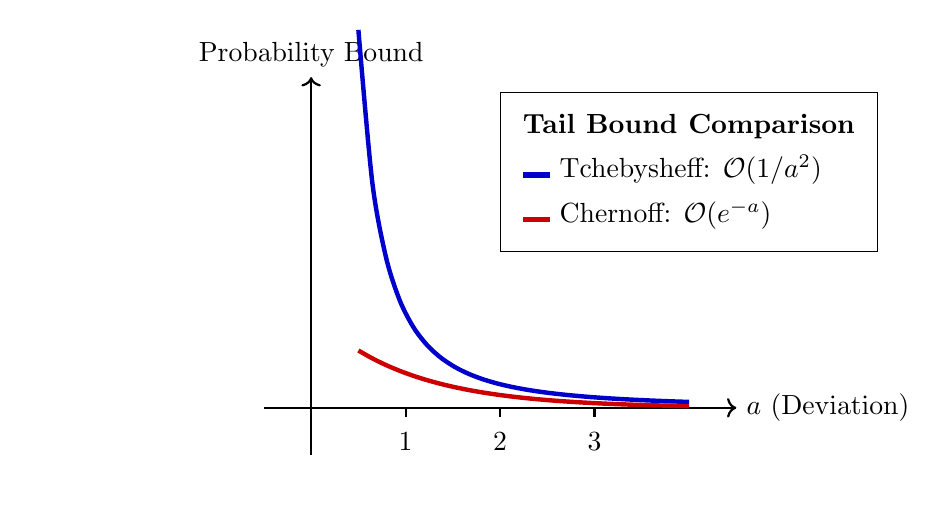
\begin{tikzpicture}[scale=1.2]
    % Background fill
    \fill[white] (-3,-1) rectangle (5,4);
    
    % Axes
    \draw[->, thick] (-0.5,0) -- (4.5,0) node[right] {$a$ (Deviation)};
    \draw[->, thick] (0,-0.5) -- (0,3.5) node[above] {Probability Bound};
    
    % Curves
    \draw[domain=0.5:4, smooth, variable=\x, ultra thick, blue!80!black] plot ({\x}, {1/(\x*\x)});
    \draw[domain=0.5:4, smooth, variable=\x, ultra thick, red!80!black] plot ({\x}, {exp(-\x)});
    
    % Labels using single node multiline rule
    \node[align=left, inner sep=8pt, anchor=west, draw, fill=white] at (2, 2.5) {
        \textbf{Tail Bound Comparison}\\[4pt]
        \textcolor{blue!80!black}{\rule{10pt}{2pt}} Tchebysheff: $\mathcal{O}(1/a^2)$\\[4pt]
        \textcolor{red!80!black}{\rule{10pt}{2pt}} Chernoff: $\mathcal{O}(e^{-a})$
    };
    
    % Tick marks
    \draw[thick] (1,0) -- (1,-0.1) node[below=2pt] {$1$};
    \draw[thick] (2,0) -- (2,-0.1) node[below=2pt] {$2$};
    \draw[thick] (3,0) -- (3,-0.1) node[below=2pt] {$3$};
\end{tikzpicture}
\end{center}
\end{proof}

\newpage

\section{Concept Checklist \& Question Mapping (Reference)}

\renewcommand{\arraystretch}{1.5}
\begin{table}[h!]
\centering
\begin{tabularx}{\textwidth}{>{\raggedright\arraybackslash}p{0.7\textwidth} >{\centering\arraybackslash}X}
\toprule
\textbf{Theoretical Concept / Proof Technique} & \textbf{Problem(s)} \\
\midrule
C1: MGF Derivation \& Convergence Constraints (Improper Integrals) & 1, 2, 4 \\
C2: Moment Extraction via Differentiation ($k$-th derivative) & 5, 30 \\
C3: Linear Transformations of MGFs & 6, 7 \\
C4: Distribution Identification via Isomorphism (Uniqueness Theorem) & 9, 10 \\
C5: Tchebysheff's Theorem for Interval Estimation & 13 \\
C6: Tchebysheff's Theorem for Variance Constraints & 14 \\
C7: Tchebysheff vs. Exact Probability (Uniform, Normal, Exponential) & 15, 30 \\
C8: Chernoff Bounds (Exponential tail bounds, Markov's Inequality) & 16, 17, 19 \\
C9: Abstract Real-World Modeling (PAC Learning, VaR, Quant Finance) & 21, 22, 23 \\
C10: Diagnostic Testing (Existence, Exactness, Independence, LOTUS) & 3, 8, 24, 25, 26, 27 \\
C11: Set-Theoretic \& Measure-Theoretic Foundations & 11, 12, 18, 20, 28, 29 \\
\bottomrule
\end{tabularx}
\end{table}

\end{document}